\begin{figure}[h!]
  \centering
\subfloat[Example of performance on a single image.]{
\label{fig:apvst_example}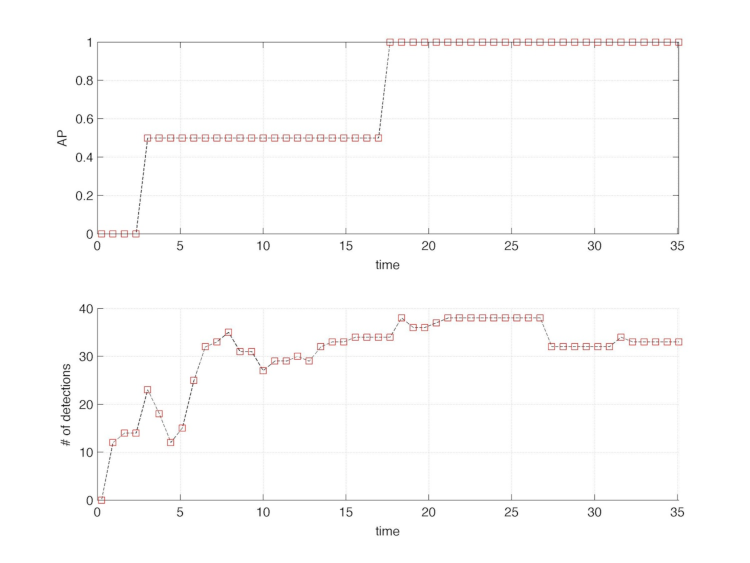
\includegraphics[width=0.75\textwidth]{../figures/example_apvst_plot.pdf}}
\\
\subfloat[Average performance across the dataset. Gray area is bounded by one standard deviation away from the mean.]{\label{fig:apvst_baseline}  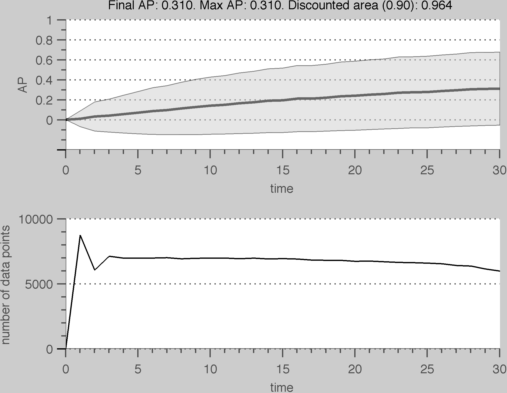
\includegraphics[width=0.75\textwidth]{../figures/apvst_baseline.png}}
  \caption{Plot of baseline performance of the Cascaded DPM Detector~\cite{Felzenszwalb2010b}, in the AP vs. Time evaluation regime.}
  \label{fig:apvst_baselines}
\end{figure}